\chapter{Data Preparation}\label{sec:data}

This study is based on simulated data produced with GEANT4~\cite{GEANT4}, using the geometric layout of the proposed Linear Collider Detector (LCD) for the CLIC accelerator~\cite{Lebrun:2012hj}. We limit the study to the central region (barrel) of the LCD detector, where the electromagnetic calorimeter (ECAL) consists of a cylinder with inner radius of 1.5 m, structured as a set of 25 silicon sensor planes, segmented in $5.1~\times~5.1$ mm$^2$ square cells, alternated with tungsten absorber planes. In the barrel region, the hadronic calorimeter (HCAL) sits behind the ECAL, at an inner radius of 1.7 m. The HCAL 
consists of 60 layers of polystyrene scintillators, segmented in cells with  $3~\times~3$ cm$^2$ area and alternated with layers of steel absorbers. 

The event simulation considers the full detector layout, including the material in front of the calorimeter and the effect of the solenoidal magnetic field. From the full data we take slices centered around the barycenter of each ECAL energy deposit and we represent the ECAL and HCAL slices as 3D arrays of energy deposits in the cells. 

We consider four kinds of particles (electrons $e$, photons $\gamma$, charged pions $\pi$, and neutral pions $\pi^0$) with energies uniformly distributed between 10 and 510 GeV, and with incident angles uniformly distributed between a polar angle $\theta$ between 1.047 and 2.094 radians with respect to the beam direction.

We get the barycenter of a shower by taking the 2D projection of its energy deposit on the ECAL inner surface. Then, knowing the point of origin of the incoming particle, we use the barycenter to estimate the particle's polar and azimuthal angles $\theta$ and $\phi$. The estimated pseudorapidity $\eta$ is then computed as $\eta=-\log[\tan\frac{\theta}{2}]$. Each single-shower event is prepared by taking a slice of the ECAL in a window around the shower barycenter, as well as the corresponding HCAL slice behind. Depending on the task (generation or reconstruction), we take:
\begin{itemize}
  \item {\bf GEN dataset}: A $51 \times 51 \times 25$ cell window in the
    ECAL, for electrons in the energy range $100-200$ GeV. Used in the shower generation task.
  \item {\bf REC dataset}: A $25 \times
    25 \times 25$ cell slice of the electromagnetic calorimeter (ECAL)
    and a corresponding $11 \times 11 \times 60$ cell slice of the
    hadronic calorimeter (HCAL), for $e,~\gamma,~\pi,$~or~$\pi^0$ in the energy range $10-510$ GeV and with $\eta$ from $-0.524-0.524$. Used in the particle reconstruction task.
\end{itemize}

%%%%%%%%%%%%%%%%

Examples of an electron shower and a charged-pion shower can be seen in Figure~\ref{fig:sample}. The incoming particles enter from the top ($z=0$), at the center of the $(x,y)$ transverse plane ($x=y=25)$. The electron event has left more hits in both the ECAL and HCAL. We can also see the presence of two subtracks in the neutral pion event. % These features are characteristic of events from these two classes.

The window size for the GEN dataset has been defined in order to contain as much of the shower information as practically possible.  
Motivated by the need of reducing the memory footprint for some of the models, we used a smaller window size for the REC dataset. When training classification models on these data, a negligible accuracy increase was observed when moving to larger windows, as described in Appendix~\ref{app:window_size}.

\begin{figure*}[htbp]
\centering
%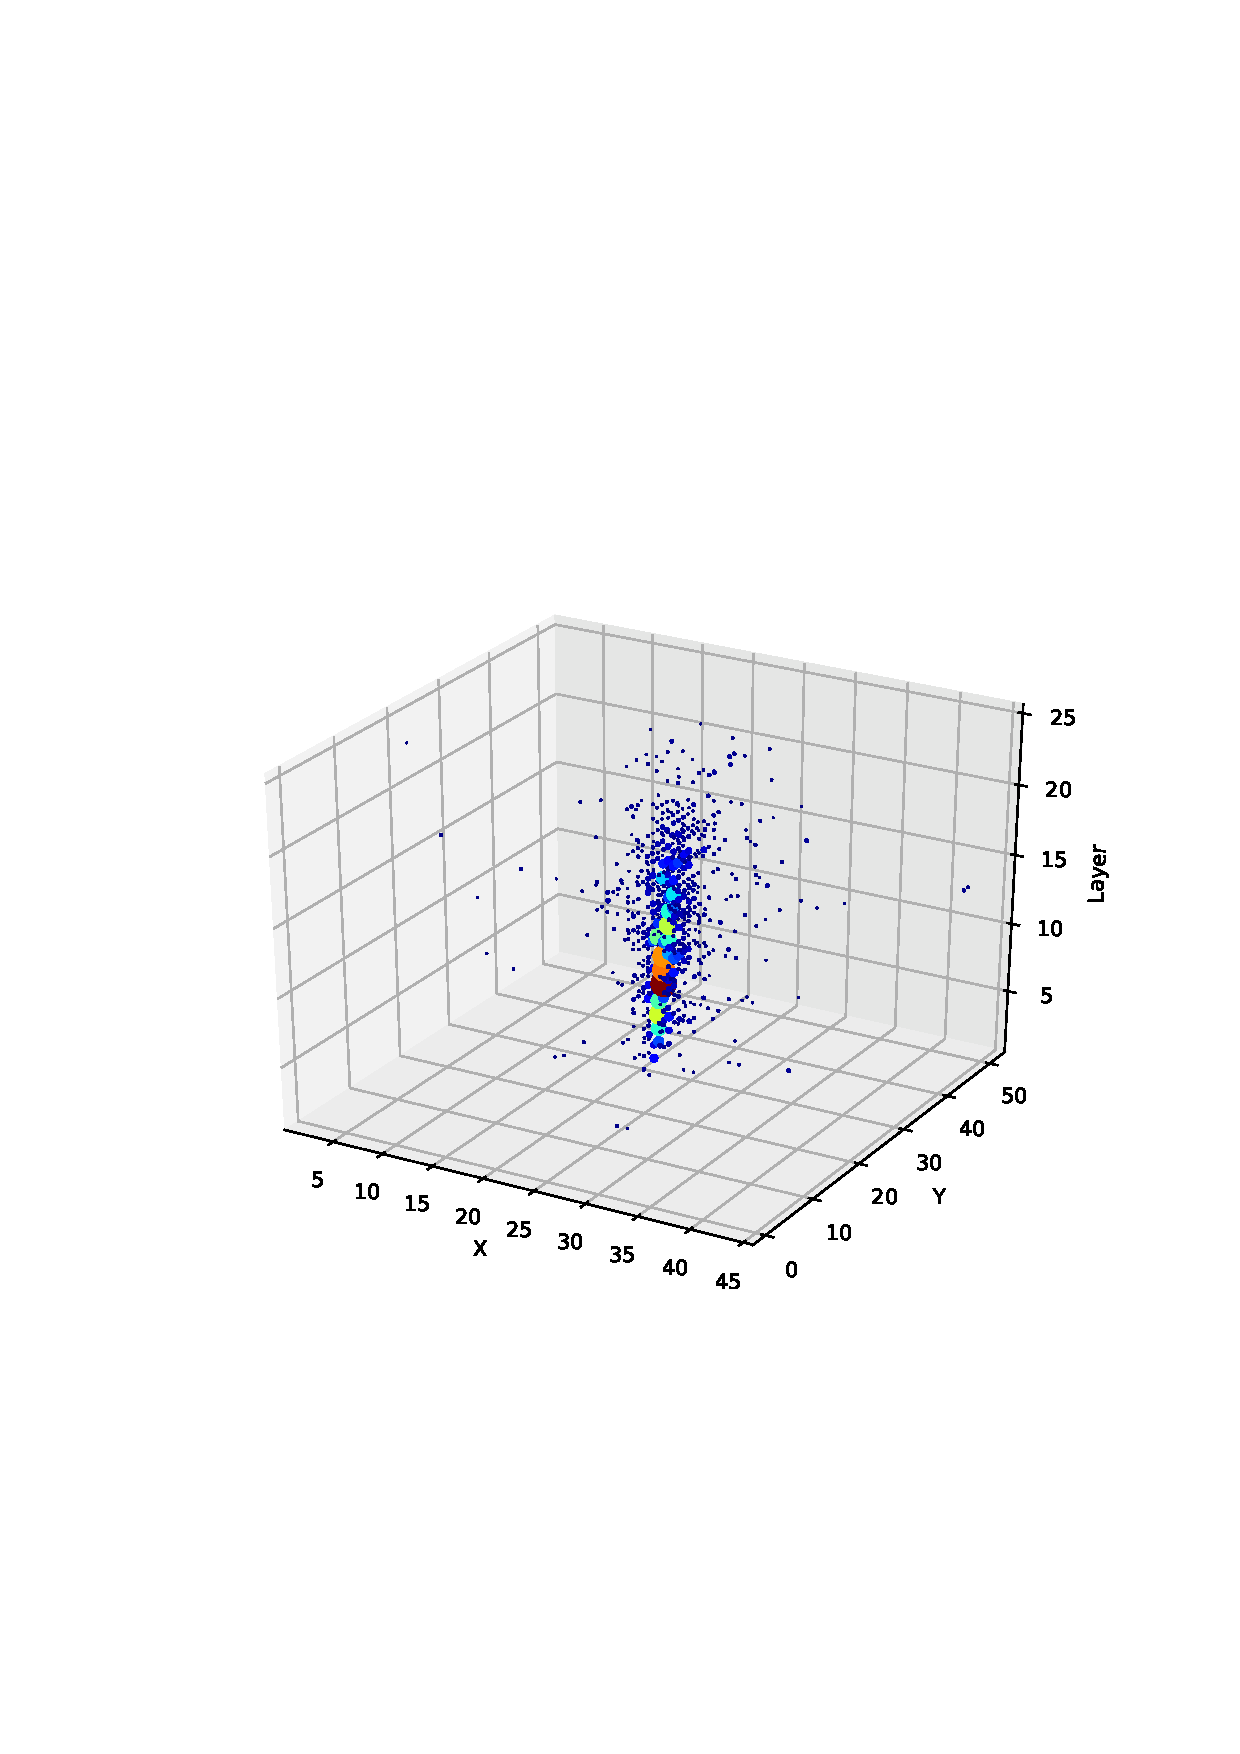
\includegraphics[width=0.45\textwidth]{images/Gamma_ECAL.pdf}
%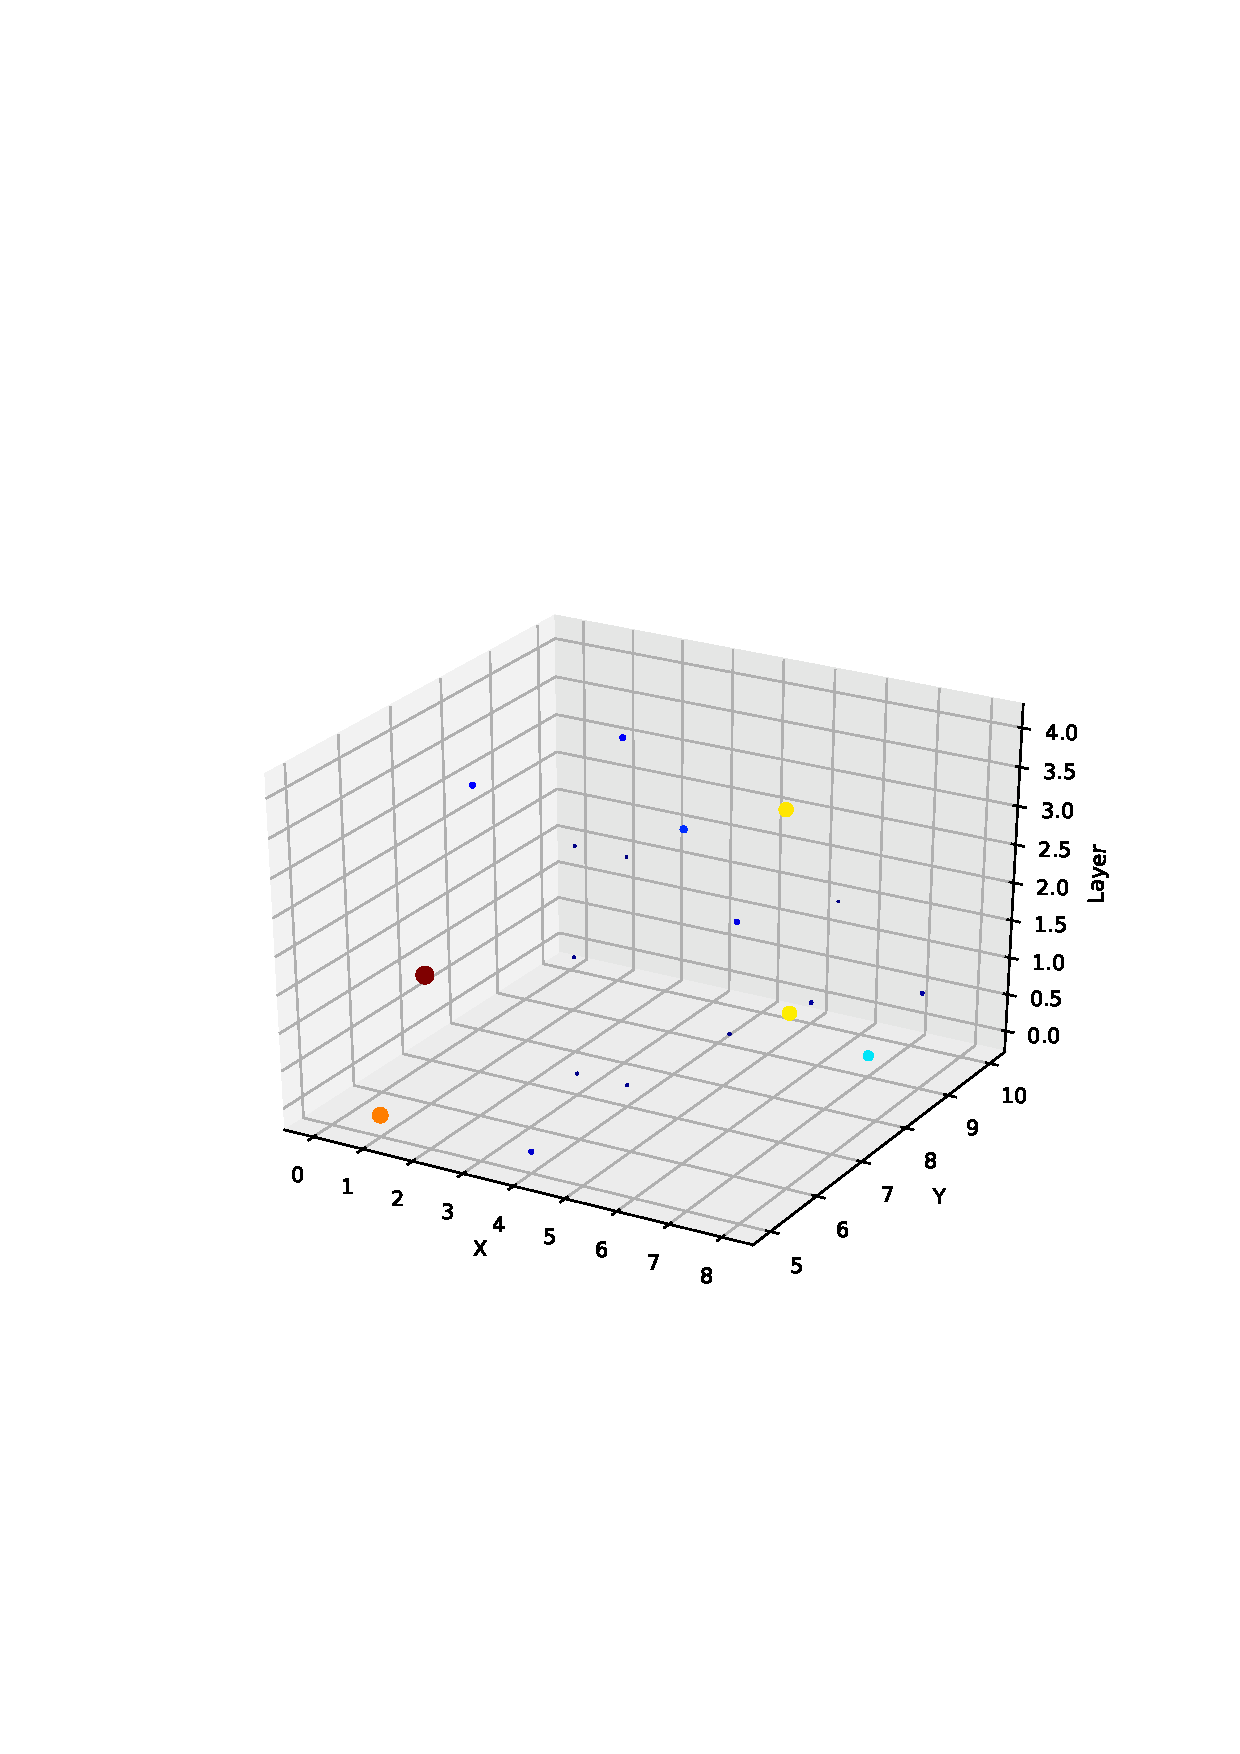
\includegraphics[width=0.45\textwidth]{images/Gamma_HCAL.pdf} \\
%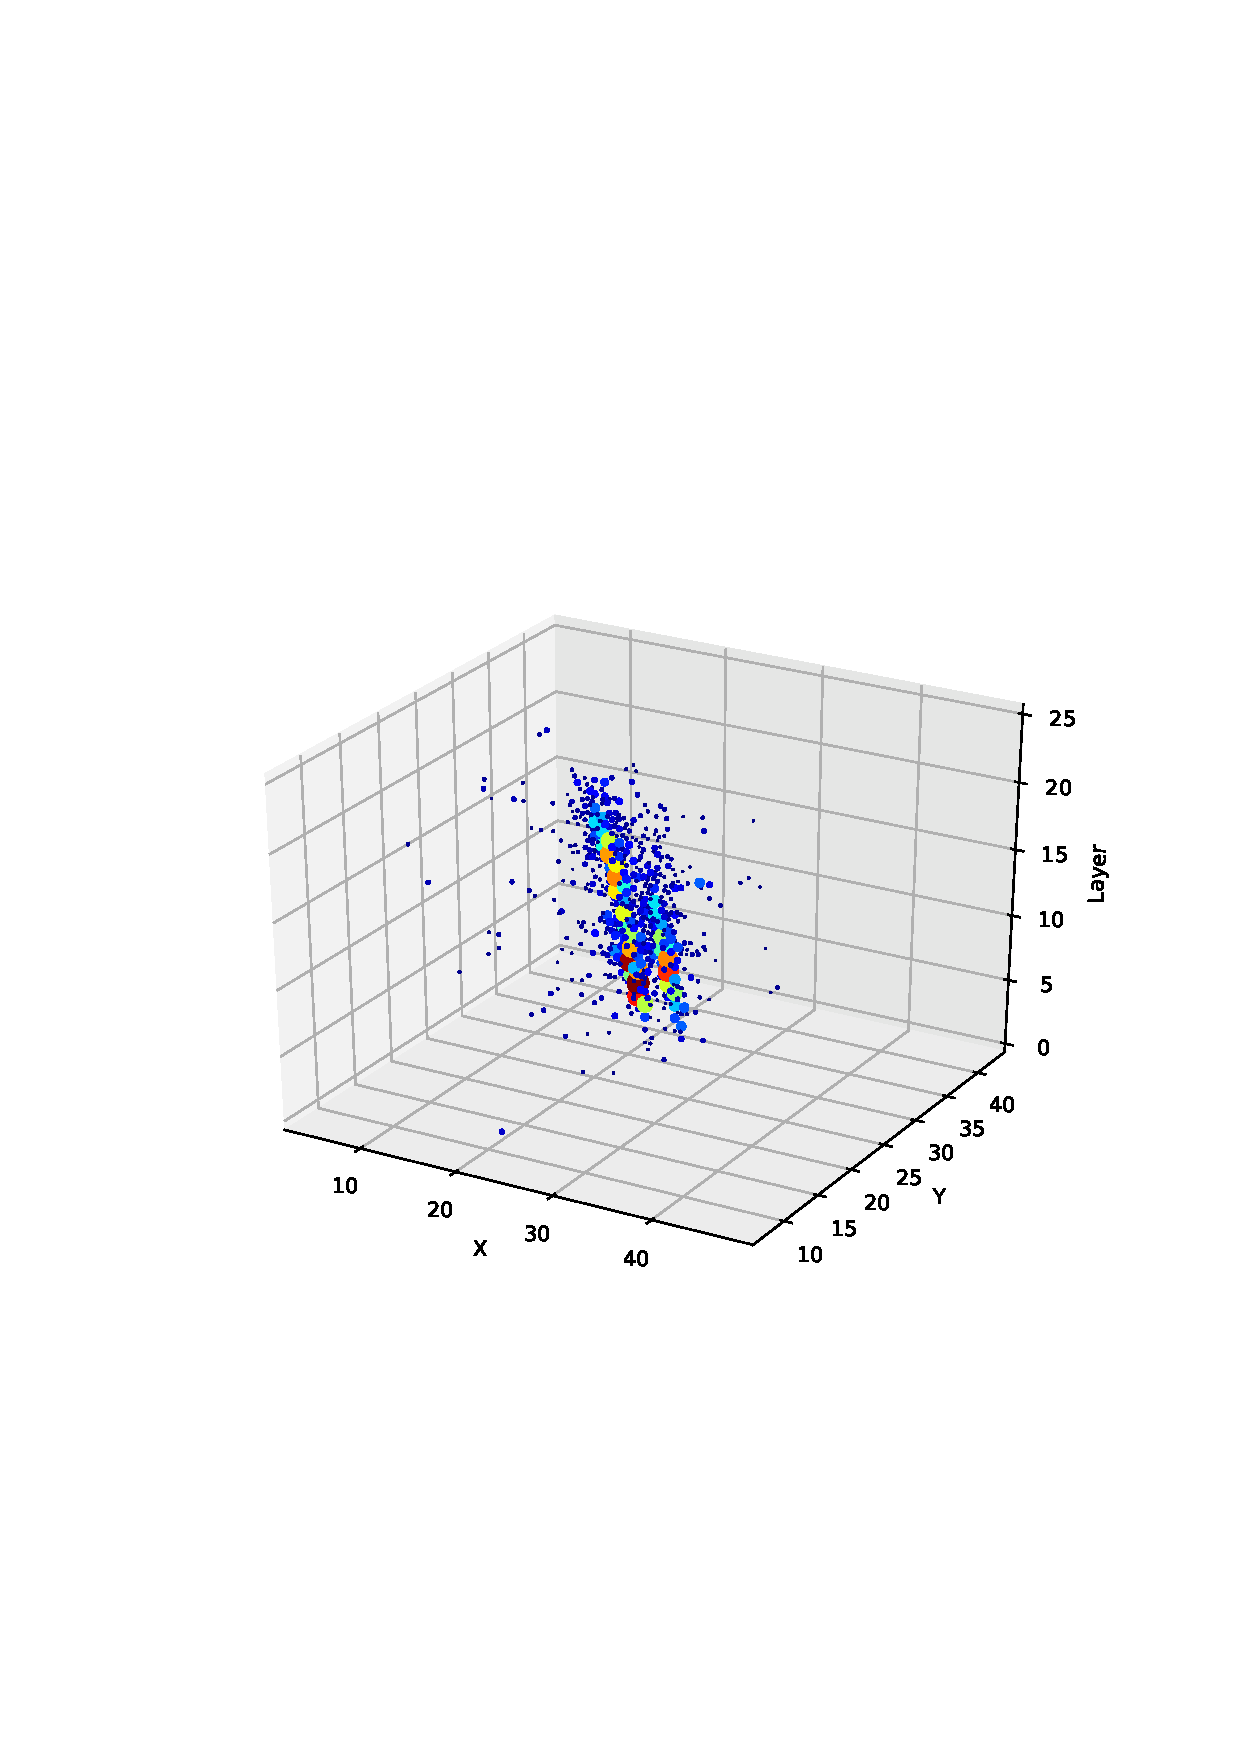
\includegraphics[width=0.45\textwidth]{images/Pi0_ECAL.pdf}
%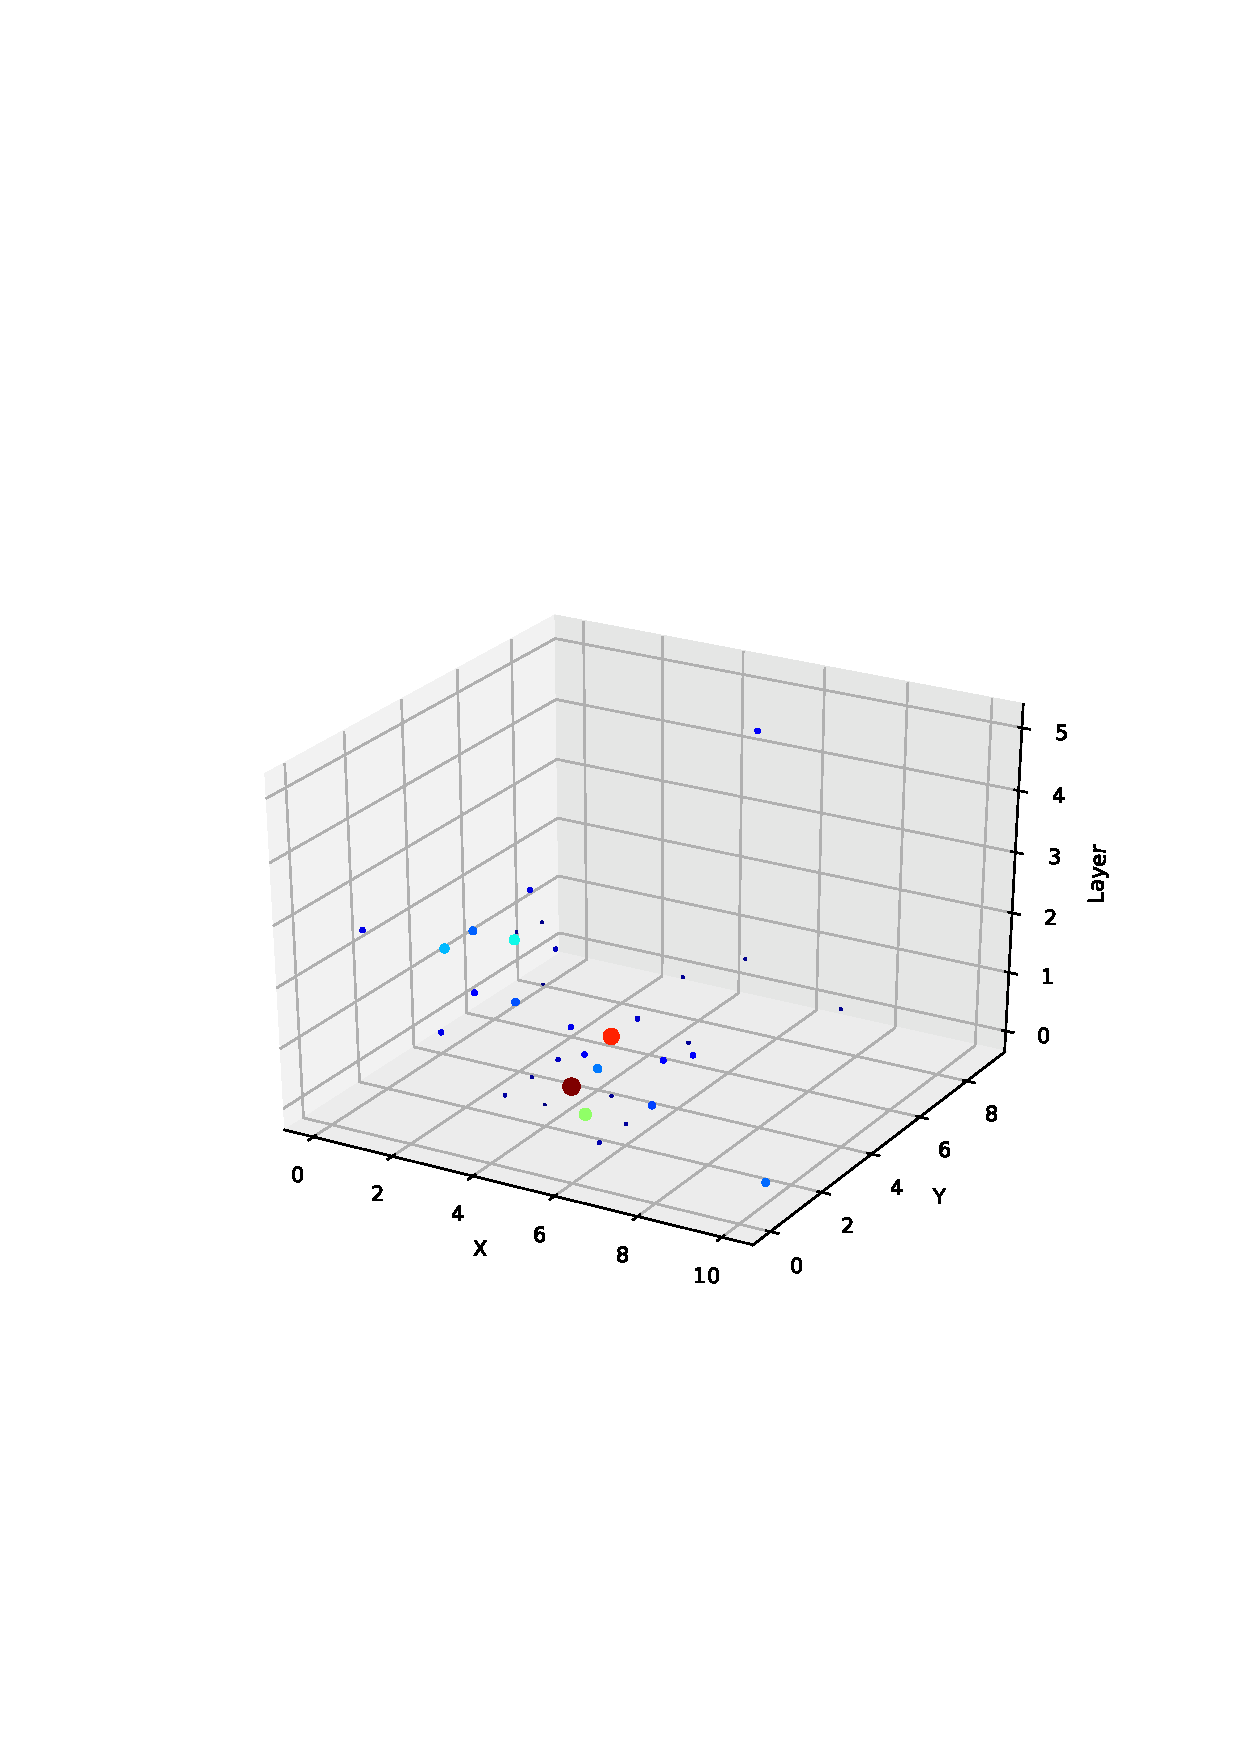
\includegraphics[width=0.45\textwidth]{images/Pi0_HCAL.pdf}
\caption{3D image of a photon (top) and neutral pion (bottom) shower in ECAL (left) and HCAL (right).}
\label{fig:sample}
\end{figure*}

%%%%%%%%%%%%%%%%%

\begin{figure}[htbp]
\centering
%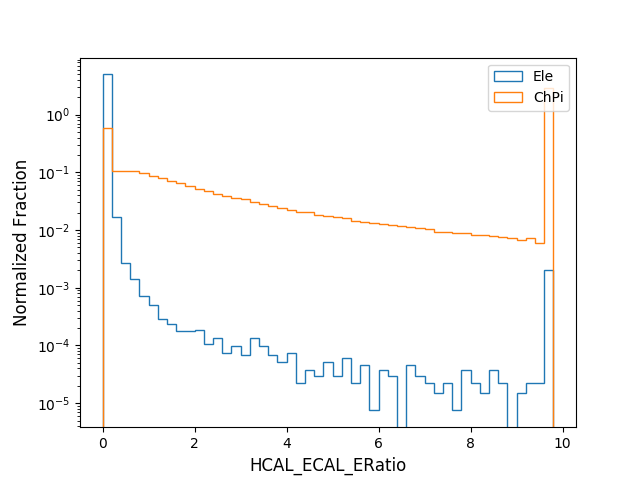
\includegraphics[width=0.3\textwidth]{images/ratios.png}
%\includegraphics[width=0.3\textwidth]{images/zoom_ratios.png}
\caption{HCAL/ECAL energy ratios for electrons and charged pions. The bottom plot is a zoomed-in version of the top plot.}
\label{fig:HE_ratio}
\end{figure}

\begin{figure}[htbp]
\centering
%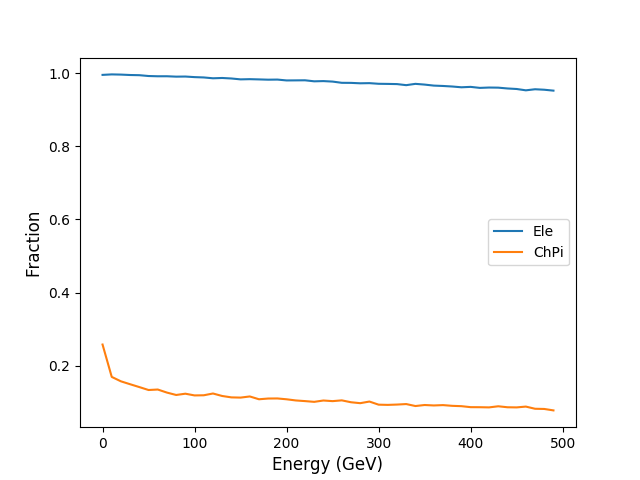
\includegraphics[width=0.3\textwidth]{images/ratio_cut_vs_energy.png}
%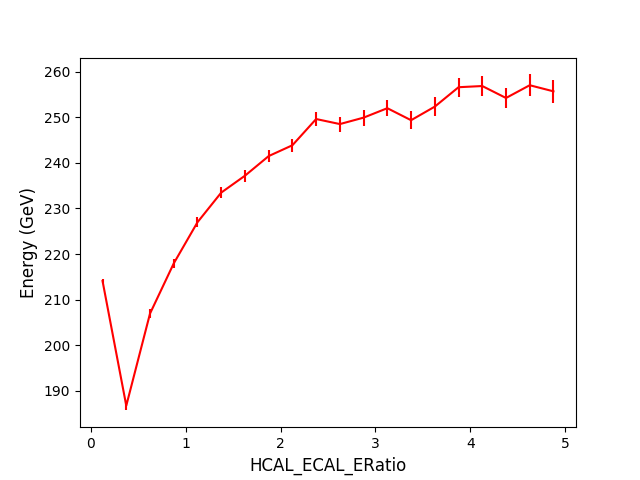
\includegraphics[width=0.3\textwidth]{images/mean_energy_vs_ratio.png}
\caption{Fractions of electrons and charged pions passing a HCAL/ECAL energy selection at various particle energies (top). The mean charged pion energy at each energy ratio (bottom).}
\label{fig:HE_ratio_energy}
\end{figure}

\begin{figure}[htbp]
\centering
%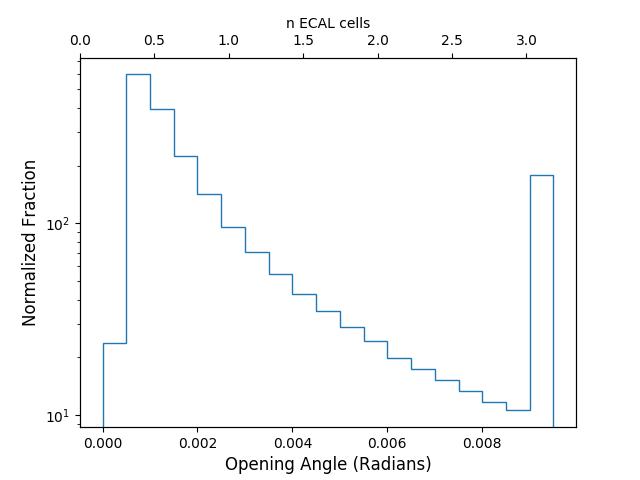
\includegraphics[width=0.3\textwidth]{images/zoom_opening_angles.png}
\caption{Opening angle distribution for neutral pions decaying into two photons.}
\label{fig:opening_angle}
\end{figure}

\begin{figure}[htbp]
\centering
%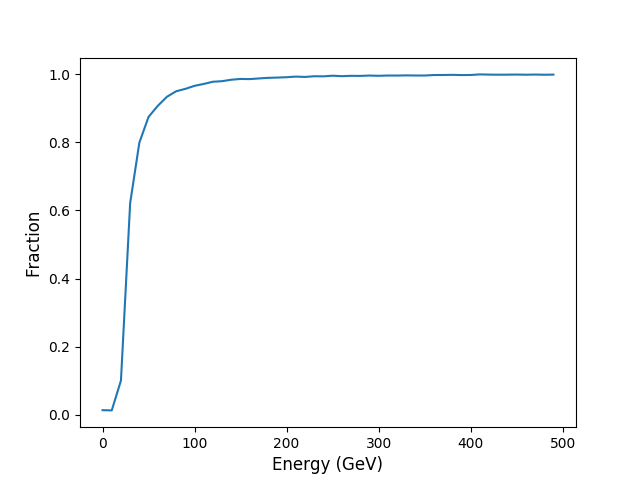
\includegraphics[width=0.3\textwidth]{images/opening_angle_cut_vs_energy.png}
%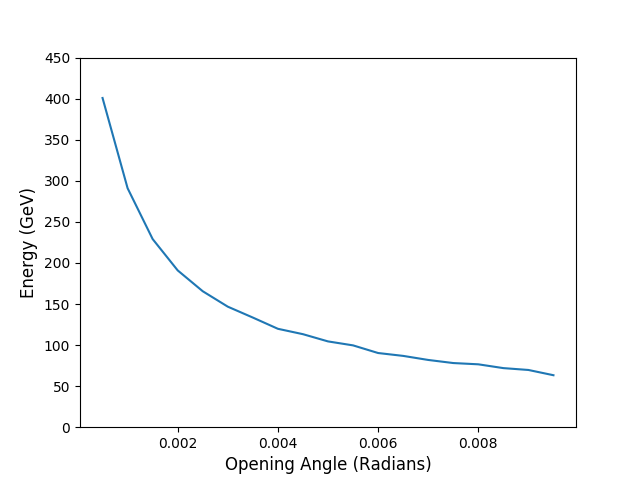
\includegraphics[width=0.3\textwidth]{images/mean_energy_vs_opening_angle.png}
\caption{The fraction of photons and neutral pions passing an opening angle < 0.01 radian selection at various particle energies (top). The mean neutral pion energy at each opening angle (bottom).}
\label{fig:opening_angle_energy}
\end{figure}

We apply a task-dependent filtering of the REC dataset, in order to select the subset of examples for which the task at hand is not trivial. For instance, distinguishing a generic pion from a generic electron is an easy task, and can be accomplished with high accuracy by looking at the HCAL/ECAL energy ratio. On the other hand, it is difficult to distinguish a generic electron from a pion that has a small HCAL/ECAL energy ratio. Thus, we ignore charged-pion showers with a large HCAL/ECAL energy ratio. To be more specific, we see in Figure~\ref{fig:HE_ratio} that the ratio of total ECAL energy to total HCAL energy is very different for electrons and charged pions, with the heavier charged pions tending to leave little energy in the ECAL. In order to make the particle-identification task more challenging, we only consider showers with HCAL/ECAL < 0.1 cut. The results of this selection are shown in Figure~\ref{fig:HE_ratio_energy}. We can see that this selection favors mostly low-energy charged pions, which tend to leave more of their energy in the ECAL rather than punching through to the HCAL. Discriminating accurately between electrons and charged pions in this range is thus crucial for compressed-mass physics analyses, where we search for decay products with low energy.

Photons and neutral pions are more similar to each other. The easily distinguishable events are mostly due to the fact that neutral pions decay into two photons which are separated by a small angle. If the pion has a low energy, the opening angle between the two photons is larger and the shower is easily identified as originating from a neutral pion. High-energy neutral pions produce more collimated photon pairs, which are more easily mistaken as a single high-energy photon. The opening angle distribution for neutral pions is shown in Figure~\ref{fig:opening_angle}. In order to limit the study to the most challenging case, we filter the neutral-pion dataset by requiring the opening angle between the two photons to be smaller than 0.01 radian.  The effect of  this requirement on the otherwise uniform energy distribution is shown in Figure~\ref{fig:opening_angle_energy}. As expected, the selection mostly removes low-energy neutral pions. 

%Generating events with these filters applied turned out to be a significant use of computing resources, especially when it came to the charged pion samples. Applying the HCAL/ECAL < 0.1 selection meant that we needed to generate several hundred times as many charged pion events as we would have needed without the filter.

The ECAL and HCAL 3D arrays are passed directly to our neural networks. We also compute a set of expert features, as described in Ref.~\cite{NIPS}. These features are used to train alternative benchmark algorithms (see Appendices~\ref{app:BDT}~and~\ref{app:regression_baseline}), representing currently-used ML algorithms in HEP.